\chapter*{Appendices}
\setcounter{section}{0}

\addcontentsline{toc}{chapter}{Appendices}
\renewcommand{\thesection}{\Alph{section}}

\section{Mathematical Preliminaries}
\label{appendix_a}
\subsection{Sets}
\subsubsection{The Axiom of Extension}
\subsubsection{The Axiom of Specification}
\subsubsection{Unordered Pairs}
\subsubsection{Unions and Intersections}
\subsubsection{Complements and Powers}
\subsubsection{Ordered Pairs}
\subsubsection{Relations}
\subsubsection{Maps}
\subsubsection{Families}
\subsubsection{Cartesian Product}
Here the symbol "$\times$" means \textbf{"Cartesian Product"} i.e. it's action w.r.t two sets $\mathbb{A}$ and $\mathbb{B}$ is the set of all ordered pairs $(a, b)$ where $a \in \mathbb{A}$ and $b \in \mathbb{B}$
\subsection{Logic}

\subsection{Complex Numbers}
\label{appendix_a}
A complex number is an ordered pair $z = \{a,b\} \in \mathbb{C}$ where $a,b \in \mathbb{R}$ where we can denote it as $z = a + ib$ where $i = \sqrt{-1}$
\subsubsection{Addition}
$z_{1} = a_{1} + ib_{1}, \ z_{2} = a_{2} + ib_{2}$
$$z_{1} + z_{2} =  (a_{1} + a_{2}) + i(b_{1} + b_{2})$$
\subsubsection{Multiplication}
$z_{1} = a_{1} + ib_{1}, \ z_{2} = a_{2} + ib_{2}$
$$z_{1}z_{2} =  (a_{1} + ib_{1})(a_{2} + ib_{2}) = (a_{1}a_{2} - b_{1}b_{2}) + i(a_{1}b_{2} + a_{2}b_{1})$$
\subsubsection{Properties}\footnote{$\mathcal{W}, \mathcal{Z}, \lambda \in \mathbb{C}$}
\subsubsubsubsection{Commutativity}
$$\mathcal{W} + \mathcal{Z} = \mathcal{Z} + \mathcal{W}$$
$$\mathcal{W}\mathcal{Z} = \mathcal{Z}\mathcal{W}$$
\subsubsubsubsection{Associativity}
$$(\mathcal{Z}_1 + \mathcal{Z}_2) + \mathcal{Z}_3 = \mathcal{Z}_1 + (\mathcal{Z}_2 + \mathcal{Z}_3)$$
$$(\mathcal{Z}_1\mathcal{Z}_2)\mathcal{Z}_3 = \mathcal{Z}_1(\mathcal{Z}_2\mathcal{Z}_3)$$
\subsubsection{Identities}
$$\mathcal{Z} + 0 = \mathcal{Z}$$
$$\mathcal{Z}1 = \mathcal{Z}$$
\subsubsubsubsection{Additive Inverse}
$$\forall \ \mathcal{Z} \ \exists \ \mathcal{Z}^{-1} \ | \ \mathcal{Z} + \mathcal{Z}^{-1} = 0$$
\subsubsubsubsection{Multiplicative Inverse}
$$\forall \  \mathcal{Z} \neq 0 \ \exists \ \mathcal{W} \ | \ \mathcal{Z}\mathcal{W} = 1$$
\subsubsubsubsection{Distributive Property}
$$\lambda(\mathcal{W} + \mathcal{Z}) = \lambda\mathcal{W} + \lambda\mathcal{Z}$$



\section{Fourier Analysis}
Fourier analysis is the study of a special set of an integral transforms. 
A fourier series is the decomposition of a general wave or oscillation into harmonic components.
Because we treat the wave vector as the independent variable of a wave, the Fourier decomposition
is typically done in terms of wave vectors. A Fourier series is a sum of sinusoidal functions, each of
which is a harmonic of some fundamental wave vector or spatial frequency. A Fourier transform is an
integral over a continuous distribution of sinusoidal functions.
A Fourier series is appropriate when the system has boundary conditions that limit the allowed
wave vectors to a discrete set. For a system where the spatial periodicity is $2L$, the Fourier decomposition of a general periodic function is the series
\begin{equation}
f(x) = \sum_{-\infty}^{\infty} c_{n}e^{i k_{n}x}
\end{equation}
where,
$$k_{n} = \frac{n \pi}{L}$$
Here $c_{n} \in \mathbb{C}$. All $f(x) \in \mathbb{R}$ can be written as:
\begin{equation}
f(x) = \frac{a_{0}}{2} + \sum^{\infty}_{n=1} \left[a_{n}\cos \left(\frac{n \pi x}{L} \right) + b_{n}\sin \left(\frac{n \pi x}{L}\right) \right]
\end{equation}
Where,
\begin{equation}
	a_{n} = \frac{1}{L} \int_{0}^{2L} f(x) \cos\left(\frac{n \pi x}{L}\right) dx
\end{equation}
\begin{equation}
	b_{n} = \frac{1}{L} \int_{0}^{2L} f(x) \sin\left(\frac{n \pi x}{L}\right) dx
\end{equation}
\begin{equation}
	c_{n} = \frac{1}{2L} \int_{0}^{2L} f(x) e^{-ik_{n}x}dx
\end{equation}
obtained by calculating the overlap integrals (i.e., projections or inner products) of the desired function with the harmonic basis functions. That is provided $f(x)$, obeys the following conditions i.e. \textbf{Dirichlet conditions}:
\begin{itemize}
\item It must be absolutely integrable over a period.
\item It must be of bounded variation in any given bounded interval.
\item It must have a finite number of discontinuities in any given bounded interval, and the discontinuities cannot be infinite.
\end{itemize}
A Fourier transform is appropriate when the system has no boundary conditions that limit the allowed wave vectors. In this case, the Fourier decomposition is an integral over a continuum of wave vectors:
\begin{equation}
	f(x) = \frac{1}{\sqrt{2 \pi}} \int_{-\infty}^{\infty} a(k)e^{ikx}dk
\end{equation}
where  the  expansion  function  $a(k)$  is  complex. To  obtain  the  expansion  function  $a(k)$  for  a  givenspatial function $f(x)$ requires the inverse Fourier transform
\begin{equation}
	a(k) = \frac{1}{\sqrt{2 \pi}} \int_{-\infty}^{\infty} f(x)e^{-ikx}dx
\end{equation}
which is a projection of the spatial function $f(x)$ onto the harmonic basis functions $e^{ikx}/\sqrt{2 \pi}$. The basis functions are orthogonal and normalized in the Dirac sense, which means their projections onto each other are Dirac delta functions
\begin{equation}
\begin{split}
	\frac{1}{2 \pi} & \int_{-\infty}^{\infty} e^{ik^{'}x}e^{-ikx}dx = \delta(k-k^{'})\\
	\frac{1}{2 \pi} & \int_{-\infty}^{\infty} e^{ikx^{'}}e^{-ikx}dk = \delta(x-x^{'})
\end{split}
\end{equation}
\subsection{Parseval’s theorem}
Parseval’s theorem states that the power is the same whether calculated in position space or wave-vector space:
\begin{equation}
\int^{\infty}_{-\infty} \abs{f(x)}^{2}dx = \int^{\infty}_{-\infty} \abs{a(k)}^{2}dk
\end{equation}

\section{The Dirac Delta Function}
\subsection{The Divergence of $\frac{\hat{r}}{r^{2}}$}
We can see why the divergence is,
\begin{equation}
\nabla . \frac{\hat{r}}{r^{2}} = 0
\end{equation}
But if we calculate this using the Divergence theorem, we find that ,
\begin{equation}
	\oint v .da = \int \left( \frac{\hat{r}}{r^{2}} \right) . \left( r^{2} \sin(\theta) d \theta d \phi \hat{r} \right) = \left( \int_{0}^{\pi} \sin(\theta) d \theta \right) \left( \int_{0}^{2\pi} d \phi \right) = 4 \pi
\end{equation}
This is paradoxical. The issue is that it blows up at $r=0$ but is is neglible everywhere else. How do we fix this? The Dirac Delta functional!
\subsection{The One-Dimensional Dirac Delta Functional}
The Dirac Delta is a functional \footnote{An object that is a map between functions} which we define as,
\begin{equation} \label{deltadef}
\delta(x-a)= 
\begin{cases}
0, & \text{if } x \neq a\\
\infty,              & \text{if } x = a
\end{cases}
\end{equation}
\begin{equation}
\int_{- \infty}^{+ \infty} \delta(x-a) dx = 1
\label{del2}
\end{equation}
$\forall \  a \in \mathbb{R}$
We can visualize it as a sharp peak at $a$,
\begin{figure}
	\centering
	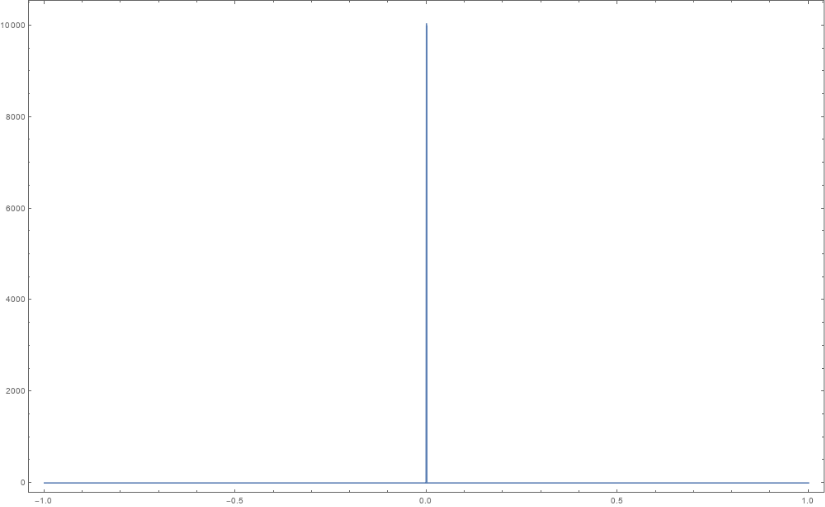
\includegraphics[scale=0.5]{Figures/delta-distribution.png}
	\caption{A Plot of $\delta(x)$}
\end{figure}
We can interpret \ref{del2} as saying "the area of the delta distribution is always 1".
\begin{equation}
f(x)\delta(x - a ) = f(a)
\end{equation}
We can combine these to get,
\begin{equation}
\int_{- \infty}^{+ \infty} \delta(x-a) f(x) dx = f(a)
\end{equation}
\subsubsection{A few interesting properties}
\begin{equation}
\delta(kx) = \frac{1}{|k|}\delta(x)
\end{equation}
\begin{equation}
\frac{d}{dx}(\delta(x)) = -\delta(x)
\end{equation}
where k is a constant
\begin{equation}
\frac{d \theta}{dx} = \delta(x)
\end{equation}
Where $\theta$ is the step function defined as,
\begin{equation}
\theta(x)= 
\begin{cases}
1, & \text{if } x > 0\\
o,              & \text{if } x \leq 0
\end{cases}
\end{equation}

\subsection{The Three-Dimensional Dirac Delta Function}
We generalize (\ref{deltadef}) to three dimensions,
\begin{equation}
\delta^{3}(\vec{r} - \vec{a}) = \delta(x-a_{x})\delta(y-a_{y})\delta(z-a_{z})
\end{equation}
\begin{equation}
\int_{- \infty}^{+ \infty} \delta^{3}(\vec{r} - \vec{a}) dV = 1
\end{equation}
We can also define the three-dimensional delta function as
\begin{equation}
\delta^{3}(\boldscriptr) = \frac{1}{4 \pi} \left[\nabla \cdot \left( \frac{\hat{\boldscriptr}}{{\scriptr	}^{2}}\right)\right]
\end{equation}
Since,
$$\nabla \left(\frac{1}{\scriptr}\right) = -\frac{\hat{\boldscriptr}}{\scriptr^{2}}$$
We can rewrite as,
\begin{equation}
\delta^{3}(\boldscriptr) = -\frac{1}{4 \pi} \left[\nabla^{2}  \left( \frac{1}{\scriptr}\right)\right]
\end{equation}
\subsection{Integral representation}
We have the relationship for the Fourrier transform,
\begin{equation}
F(x) = \int f(t) e^{-ixt} dt
\end{equation}
and it's inverese
\begin{equation}
f(t) = \frac{1}{2 \pi} \int F(x) e^{ixt} dx
\end{equation}
Plugging in Eq. into Eq. we find that 
\begin{equation}
	F(y) = \frac{1}{2 \pi} \int_{-\infty}^{\infty} F(x) dx \int_{-\infty}^{\infty}e^{i(x-y)t} dt
\end{equation}	
Now, invoking the definig property of the Delta function,
\begin{equation}
F(y) = \int_{-\infty}^{\infty} F(x) \delta(x-y) dx
\end{equation}
Comparing and we find that,
\begin{tcolorbox}
\begin{equation}
\delta(x-y) = \frac{1}{2 \pi} \int_{-\infty}^{\infty} e^{i(x-y)t} dt
\end{equation}
\end{tcolorbox}

\section{Linear Algebra}
\label{appendix_a}
\subsection{Vector Spaces}
A linear vector space or simply a vector space $\mathbb{V}$ is a set along with the multiplication $(.)$ and addition $(+)$ operations over a field $\mathcal{F}$, such that the following axioms hold:
\begin{itemize}
	\item \textbf{Commutativity:} $\ket{u} + \ket{v} = \ket{v} + \ket{u}$
	\item \textbf{Associativity:} $(\ket{u} + \ket{v}) + \ket{w} = \ket{v} + (\ket{u} + \ket{w})$
	\item \textbf{Additive Identity:} 
	$\exists \  \ket{0} \in \mathbb{V} \ | \ \ket{v} + \ket{0} = \ket{0} + \ket{v} = \ket{v}$
	\item \textbf{Additive Inverse:} $\forall \ \ket{v} \ \exists \ \ket{v^{-1}} \ | \ \ket{v} + \ket{v^{-1}} = 0$
	\item \textbf{Multiplicative identity:} $\exists \ 1 \in \mathbb{V} \ | \ 1 .\ket{v} = \ket{v}$
	\item \textbf{Multiplicative Associativity:}  $(\alpha \beta) \ket{v} = \alpha (\beta \ket{v})$
	\item \textbf{Distributive Properties:} 
	\begin{itemize}
		\item $(\alpha + \beta) \ket{u} = \alpha \ket{u} + \beta \ket{u}$
		\item $\alpha (\ket{u} + \ket{v}) = \alpha \ket{u} + \alpha \ket{v}$
	\end{itemize}
\end{itemize}
Here, $\alpha , \beta \in \mathcal{F}$ and $\ket{u}, \ket{v} $ and $\ket{w} \in \mathbb{V}$
\subsection{Subspaces}
Given a vector space $\mathbb{V}$, a subset of its elements that form a vector space among themselves is called a subspace. We will denote a particular subspace $i$ of dimensionality $n_{i}$ by $\mathbb{V}^{n_{i}}_{i}$.\\
   Given two subspaces, and , we define their sum $\mathbb{V}^{n_{i}}_{i} \oplus \mathbb{V}^{m_{i}}_{i} = \mathbb{V}^{l_{i}}_{i}$ as the set containing:
\begin{enumerate}
\item All the elements of $\mathbb{V}^{n_{i}}_{i}$
\item All the elements of $\mathbb{V}^{m_{j}}_{j}$
\item And all possible linear combinations of the above
\end{enumerate} 
However for the elements of (3), closure is lost. The dimensionality of such a subspace is $n + m$.
\subsection{Bases, Span and Linear Independence}
\begin{itemize}
    \item If $S = \{\ket{v}_{1},\ket{v}_{1},...,\ket{v}_{k}\} \subset \mathbb{V}$ is a set of $k$ vectors in $\mathbb{V}$, then the span of $S$, denoted $Span \{\ket{v}_{1},\ket{v}_{2},...,\ket{v}_{k} \}$ or Span S, is defined to be just the set of all vectors of the form $\{c^{1}\ket{v}_{1} + c^{2}\ket{v}_{2} + .... + c^{k}\ket{v}_{k} \}$
    \item Such vectors are known as linear combinations of the $v_i$, so Span $S$ is just the set of all linear combinations of the vectors in $S$
    \item A basis for a vector space $\mathbb{V}$ is a linearly independent set $\mathcal{B} \subset \mathbb{V}$ whose span is all of $\mathbb{V}$
    \item The dimension of a vector space $\mathbb{V}$, denoted $dim \ \mathbb{V}$ , is the number of
elements of any finite basis
\item If no finite basis exists, then we say that $\mathbb{V}$ is infinite dimensional.
\item Components are simply the scalar coefficients with respect to a specific basis
\item Vectors exist independently of any chosen basis
\item Vectors transform (contravairant) in the opposite way (the inverse of the original transformation matrix) to which it's basis transforms (covariant)
\end{itemize}

\subsection{Linear Maps}
A linear map/transformation is simply transformation $\hat{L}$ that
		\begin{itemize}
				\item Adds inputs or outputs, $\hat{L}(\ket{v} + \ket{w}) = \hat{L}(\ket{v}) + \hat{L}(\ket{w})$
			\item Scale the inputs or outputs, $\hat{L}(\alpha \ket{v}) = \alpha \hat{L}(\ket{v})$
		\end{itemize}
		Here, $\alpha  \in \mathcal{F}$ and $\ket{v} $ and $\ket{w} \in \mathbb{V}$
\subsection{Hermitian Forms}
Every vector space $\mathbb{V}$ has a dual space $\mathbb{V}^{*}$
\begin{itemize}
\item $\forall \ \ket{v} \ \exists \ \bra{w} := \ket{v} \rightarrow \mathbb{R}$
\item Much like a vector space, one can assign the dual space a Basis set $e^{i}$
\item It is common to set the basis up in a way that $$e^{i}(e_{j}) = \delta^{i}_{j} = \begin{cases}            1, &         \text{if } i=j,\\
            0, &         \text{if } i\neq j.
    \end{cases}$$
\end{itemize}
A non-degenerate Hermitian form on a vector space $\mathbb{V}$ is a function
$\langle \cdot | \cdot \rangle$ which assigns to an ordered pair of vectors $\ket{v}, \ket{w} \in \mathbb{V}$ a scalar, denoted $\braket{v}{w}$,
having the following properties:
\begin{itemize}
    \item \textbf{Linearity for the vectors:} $\bra{U}(\alpha\ket{V}+\beta\ket{W}) = \bra{U}\alpha\ket{V} + \bra{U}\beta\ket{W} = \alpha\braket{U}{V} + \beta\braket{V}{W}$
    \item \textbf{Hermicity/Skew-symmetry:} $\braket{V}{W} = {(\braket{W}{V})}^{*}$
    \item \textbf{Non-degeneracy:} For each $\ket{v} \neq 0 \in \mathbb{V}$, there exists $w \in \mathbb{V}$ such that $\braket{v}{w} \neq 0$
    \item \textbf{Positive-Definiteness:} $\braket{V}{V} > 0$, for all $\ket{V} \neq \ket{0}$
\end{itemize}
\begin{itemize}
    \item There exists a symmetric bilinear function $g$ that maps Vectors to Duals i.e. $g : = \ket{v} \rightarrow \bra{v}$
    \item $\bra{v}$ is termed the metric dual
\end{itemize}

\subsection{Kernels}
For any linear map $\hat{T}$, a Kernel is a set of all vectors whose image is the zero vector. We often denote this space as $Ker(\hat{T})$.

%\subsection{Inner Product}
%A (sesquilinear i.e. half-linear) inner product is a generalization of the dot product that we are familiar with. It is defined as follows, the operation $\langle . | . \rangle$
%\begin{itemize}
 %   \item \textbf{Skew-symmetry:} $\langle V | W \rangle = { \langle W | V \rangle}^{*}$
  %  \item \textbf{Positive semidefiniteness:} $\langle V | V \rangle \geq 0$,* unless and until *$| V \rangle = | 0 \rangle$
   % \item \textbf{Linearity for the vectors:} $\langle U | (\alpha | V \rangle+\beta | W \rangle) = \langle U | \alpha | V \rangle + \langle U | \beta | W \rangle = \alpha \langle U |  V \rangle+ \beta \langle V |  W \rangle$*
%\end{itemize}
%Where, $\alpha \in \mathbb{C}$ and $| U \rangle,| V \rangle,| W \rangle \in \mathbb{V}$ and $\langle U| ,\langle V |, \langle W| \in \mathbb{V}^{*}$

\subsection{Hilbert Spaces}
A Hilbert space is an inner product vector space $\mathcal{H}$ that
\begin{itemize}
    \item has an norm i.e. length defined as $||V|| =  \sqrt{\langle V | V\rangle}$
    \item  is complete i.e. all of it's Cauchy sequences converge
\end{itemize}
A Cauchy sequence is simply a sequence of numbers whose succeeding term is smaller than the preceding one and when taken to a limit it converges. That is if you have a sequence One can visualize this as the plot of a dampened oscillator.

\subsection{Tensors}
A tensor is defined as a multilinear i.e. linear in every argument map $T(r,s)$ of the form
\begin{equation}
    \underbrace{V \times V \times V \times ...}_\text{your comment} \times \underbrace{V^{*} \time V^{*} \time V^{*} \times ...}_\text{s-times} \rightarrow \mathbb{R}
\end{equation}
\subsection{The Tensor Product}
A tensor product operation of two vectors $V \otimes W$ is defined as a bilinear function that maps $V^{*} \times W^{*}$ to the underlying field whose action is defined as
\begin{equation}
    (v \otimes w)(h,g) = v(h)w(g) \ \forall \ h \in V^{*}, g \in W^{*}
\end{equation}
Often times, a tensor is simply the set of all coefficients put in a matrix for such a map.
\subsection{A few interesting tensors}
\subsubsection{Kronecker delta}
It simply has the ‘function’ of ‘renaming’ an index:
$$\delta^{\mu}_{\nu} x^{\nu} = x^{\mu}$$
it is in a sense simply the identity matrix.
\subsubsection{Levi-Civita Pseudotensor}
\label{Levi}
The Levi-Civita Pseudotensor i.e. Tensor density is a completely anti-symmetric i.e. $\epsilon_{ijk} = -\epsilon_{jik} = -\epsilon_{ikj} = -\epsilon_{kji}$, we define it as:
\begin{equation}
\epsilon_{ijk} = \begin{cases}
1 \ \text{if } ijk \text{ is an even permuation of } 123\\
-1 \ \text{if } ijk \text{ is an odd permuation of } 123\\
0  \text{ if two indices are equal}\\
\end{cases}
\end{equation}
We have the identity
\begin{equation}
\epsilon_{\alpha \beta \nu}\epsilon_{\alpha \beta \sigma} = \delta_{\mu \rho} \delta_{\nu \sigma} - \delta_{\mu \sigma}\delta_{\nu \rho}
\end{equation}
From this it follows that,
\begin{equation}
\epsilon_{\alpha \beta \nu}\epsilon_{\alpha \beta \sigma} = 2\delta_{\nu \sigma}
\end{equation}
and
\begin{equation}
\epsilon_{\alpha \beta \gamma}\epsilon_{\alpha \beta \gamma} = 6
\end{equation}
Using these identities and the definition we can rewrite the cross-product of two vectors as,
\begin{equation}
\vec{a} = \vec{a} \cross \vec{b}  = \epsilon_{ijk}a_{j}b_{k}
\end{equation}
Thus the expressions in vector product notation can be changed to index notation for example,
$$
c = \nabla.(\nabla \cross \vec{a}) = \nabla_{i}(\epsilon_{ijk}\nabla_{j}a_{k}) = \epsilon_{ijk}\partial_{i}\partial_{j}a_{k}
$$
because,
$$\nabla_{i} = \frac{\partial}{\partial x_{i}} := \partial_{i}$$

\section{Complex Analysis}
\label{appendix_c}
\subsection{Analytic Functions}
A complex valued function, 
\begin{equation}
    f(z) = u(x,y) + iv(x,y)
\end{equation}
for $z = x + iy$ is said to be analytic in a region close to a point $z$, then it has a derivative at every point in that region i.e. neighbourhood. We define it's derivative as:
\begin{equation}
   f^{'}(z)  = \frac{df}{dz} = \lim_{\delta z  \rightarrow 0}\frac{\delta f(z + \delta z) - f(z)}{\delta z}
\end{equation}
An important point here is that $f^{'}(z)$ should not depend on the way $\delta z$ is selected. An alternate way to state this is to mandate that the Cauchy-Riemann relations,
\begin{equation}
    \begin{aligned}
    \frac{\partial u}{\partial x} = \frac{\partial v}{\partial y} \\
    \frac{\partial v}{\partial x} = - \frac{\partial u}{\partial y}
    \end{aligned}
\end{equation}
hold for $f(z)$.
\subsection{Poles}
A pole is a type of singularity i.e. a point where a mathematical object is not defined
. Think of the function $1/ z^{n}$ at $z = 0$. Let's suppose a function $f(z)$ is analytic between $C_{1}$ and $C_{2}$. In the region between them we can expand out $f(z)$ about a point $z_{0}$ as a Laurent series
\begin{equation}
    f(z) = a_{0} + a_{1} {(z- z_{0})} + a_{2} {(z- z_{0})}^{2} + ... + \frac{b_{1}}{{(z- z_{0})}} + \frac{b_{1}}{{(z- z_{0})}^{2}} + ...
\end{equation}
The part of the series with the b coefficients is termed as the principal part of the series. From this we can draw a few conclusions:
\begin{itemize}
    \item If all $b_{i}$'s are zero then $f(z_{0})$ is analytical at $z = z_{0}$
    \item If all $b_{i}$'s after $b_{n}$ are zero then we can say 
\end{itemize}
\subsection{Contour Integrals}
A contour $C$ is a closed path in $\mathbb{C}$ with a finite number of corners that doesn't cross itself. We will now review interesting things about integrals around such contours as, often we want to do difficult integrals over real variables. These may
be turned into easier integrals if we form a contour in the complex plane
which includes the original domain of integration which turn out to be much more tractable. The art is in choosing the best contour to do the integral
\subsubsection{Cauchy's Theorem}
If $f(z)$ is analytic on and inside $C$, then
\begin{equation}
    \oint_{C} dz \ f(z) = 0
\end{equation}
\subsubsection{Cauchy's Integral Formula}
If $f(z)$ is analytic on and inside a simple closed curve $C$ and a point a inside the curve, then 
\begin{equation}
    f(a) = \frac{1}{2 \pi i} \oint_{C} dz \frac{f(z)}{z-a}
\end{equation}
\subsubsection{Residue Theorem}
If $f(z)$ has singularities at points $z_{i}$, then for a contour $C$ that encloses them we have
\begin{equation}
    \oint_{C}dz \ f(z) = 2 \pi i \sum_{i} \text{Residue} \ \text{at} \ f(z_{i}) \ \text{inside} \ C
\end{equation}
wherein the integral is evaluated anti-clockwise i.e. we do it clockwise and simply invert the sign
\subsection{Branch Cuts}

\subsection{Cauchy's Principal Value Method}

\section{Group Theory}
\label{appendix_d}
\subsection{Preliminaries}
\subsubsection{Definition of a Group}
Examples of groups: 
\subsubsection{Subgroup}
For a group $G(G, *)$, a subgroup $H \subseteq G$ is defined as a group with the same composition binary operator. The notation $H \leq G$ is often used to indicate that $H$ is a subgroup of $G$
\subsubsection{Multiplication Tables}
From this itself we can tell if a group is abelian, as an abelian group would have 
\subsubsection{Morphisms}
A \textbf{group homomorphism} $\phi : G \rightarrow H$ is a map between two groups $G(G, *)$ and $H(H, +)$ that preserves the group structure i.e.
\begin{equation}
    \phi(a * b) = \phi(a) + \phi(b) \ \forall \  a,b \in G
\end{equation}
This preserves the group structure because:
\begin{itemize}
    \item This maps identity elements to identity elements i.e. $\phi(e_G) = e_{H}$
    \item 
\end{itemize}
The \textbf{Kernel} of a group homorphism $\phi : G \rightarrow H$ is the set of all elements of $G$ that are sent to the identity of $H$ i.e. $ker\phi = \{ g \in G | \phi(g) = e_{G}\}$
\begin{tcolorbox}
\textbf{Proposition:} A group homomorphism $\phi: G \rightarrow H$ is injective if and only if it's Kernel is trivial i.e. $ker\phi = \{ e_{G} \}$
\end{tcolorbox}
Two groups $G$ and $H$ are said to be isomorphic i.e. $G \iso H$ if there exists an invertible group homomorphism $\phi : G \rightarrow H$ i.e. an isomorphism

\subsubsection{Cosets}
\subsection{Important Theorems}
\subsubsection{Lagrange's Theorem}
\begin{tcolorbox}
    For any finite group G, the order (number of elements) of every subgroup of G is  equal to the number of of left cosets of $H$ in $G$
\end{tcolorbox}
\subsubsection{Cayleys's Theorem}
\begin{tcolorbox}
    Every group $G$ is isomorphic to a subgroup of the symmetric group acting on $G$
\end{tcolorbox}

\subsection{Lie Groups}

\subsection{Representation Theory}

\subsection{Reducibility and Irreducibility}

\section{Variational Calculus}
\subsection{A Lemma}
If,
\begin{equation}
    \int_{a}^{b}A(t)\eta(t)dt =0
\end{equation}
where,
\begin{itemize}
    \item $\eta(a) = \eta(b) = 0$
    \item $A(t)$ and $\eta(t)$ are both twice differentiable in the closed interval $[a,b]$ 
\end{itemize}
then,
\begin{tcolorbox}
$A(t) = 0$ throughout $[a,b]$
\end{tcolorbox}
\subsubsection{Proof by Contradiction}
Suppose that there exists $A(c) \neq 0$ for some $a < c < b$. For definiteness let's also suppose that $A(c) > 0$. Due to the continuity of $A(t)$, an interval $[t_{1},t_{2}]$ about c but within $[a,b]$ exists on which A(t) > 0. However under these conditions we can construct a $\eta(t)$ that leads to the integral being non-zero. For example,
\begin{equation} \label{deltadef}
\eta(t) =  
\begin{cases}
{(t-t_{1})}^{3}{(t_{2}-t)}^{3}, & \text{for } t_{1} < t < t_{2}\\
0, & \text{for } t < t_{1} \text{ and } t > t_{2}
\end{cases}
\end{equation}
\subsection{Deriving the Euler-Lagrange Equations}
The goal here is to find the extremal of the functional
\begin{equation}
			J(\alpha) = \int_{x_{2}}^{x_{1}}f\{y(\alpha , x),y^{'}(\alpha , x);x \} dx
		\end{equation}
		That is $\forall \ \eta(x)$, we want to find
		\begin{equation}
		\left. \frac{\partial J}{\partial \alpha} \right |_{\alpha = 0}  = 0
		\end{equation}
		Where $\alpha$ is a parameter.We thus start by, parameterizing $y$ as,
		\begin{equation} \label{increment}
		    y(x) = y(0) + \alpha \eta(x)
		\end{equation}
	We can now take the derivative
\begin{equation}
\frac{\partial J}{\partial \alpha} = \frac{\partial}{\partial \alpha}\int_{x_{2}}^{x_{1}}f\{y(\alpha , x),y^{'}(\alpha , x);x \} dx
\end{equation}
$$\frac{\partial J}{\partial \alpha} = \int_{x_{2}}^{x_{1}} \left(\frac{\partial f}{\partial y}\frac{\partial y}{\partial \alpha} + \frac{\partial f}{\partial y^{'}}\frac{\partial y^{'}}{\partial \alpha} \right) dx$$
From Equation (\ref{increment}) we have
\begin{align}
\frac{\partial y}{\partial \alpha} = \eta(x) \ ; \  & \frac{\partial y^{'}}{\partial \alpha} = \frac{d \eta}{d x}
\end{align}
a
	$$\frac{\partial J}{\partial \alpha} = \int_{x_{2}}^{x_{1}} \left(\frac{\partial f}{\partial y}\eta(x) + \frac{\partial f}{\partial y^{'}}\frac{\partial \eta}{\partial x} \right) dx$$	
	\begin{itemize}
		\item The second term in the integrand can be integrated by parts:
	\end{itemize}
	$$\int_{x_{1}}^{x_{2}} \frac{\partial f}{\partial y^{'}}\frac{d \eta}{dx} dx = \left \frac{\partial f}{\partial y^{'}} \eta(x) \right |^{x_{2}}_{x_{1}} -\int_{x_{1}}^{x_{2}} \frac{d}{dx} \left(\frac{\partial f}{\partial y^{'}}\right)\eta(x) dx $$
	$$\frac{\partial J}{\partial \alpha} = \int_{x_{1}}^{x_{2}} \left(\frac{\partial f}{\partial y} - \frac{d}{dx}\frac{\partial f}{\partial y^{'}} \right) \eta(x) dx$$
	\begin{tcolorbox}
		\begin{equation}
		\frac{\partial f}{\partial y} - \frac{d}{dx}\frac{\partial f}{\partial y^{'}} = 0
		\end{equation}
	\end{tcolorbox}
\subsection{Special Notation}
	We have the equation
\begin{equation}
\frac{\partial J}{\partial \alpha} d\alpha = \int_{x_{1}}^{x_{2}} \left(\frac{\partial f}{\partial y} - \frac{d}{dx}\frac{\partial f}{\partial y^{'}} \right) \frac{\partial y}{\partial \alpha} d \alpha dx = 0
\end{equation}
It can be written as 
\begin{equation}
\delta J = \int_{x_{1}}^{x_{2}} \left(\frac{\partial f}{\partial y} - \frac{d}{dx}\frac{\partial f}{\partial y^{'}} \right) \delta y \ dx = 0
\end{equation}
where
\begin{equation}
\begin{cases}
\frac{\partial J}{\partial \alpha} d\alpha = \delta J\\
\frac{\partial y}{\partial \alpha} d\alpha = \delta y
\end{cases}
\end{equation}
The condition of extremum then becomes,
\begin{equation}
\delta J = \delta \int_{x_{1}}^{x_{2}} f\{y, y^{'}; x\} dx = 0
\end{equation}
Sometimes we term this the functional derivative i.e. the Frechet derivative
\begin{equation}
    
\end{equation}
\subsection{Constraints}
\subsection{Lagrange Multipliers} 
\subsection{Variational Calculus in Physics}
\subsection{The Legendre Transform}
The Legendre transform
\subsection{The Rund-Tutman Identity}

\section{Probability Theory}
\subsection{Basics}
Probability is a number between 1 and 0 assigned to a proposition i.e. the probability of a proposition $A$
\begin{equation}
    prob(A) \in [0,1]
\end{equation}

\subsection{Discrete Distributions}
Suppose we have a frequency distribution 
\begin{equation}
N = \sum_{j=0}^{\infty} N(j)
\end{equation}
The probability of an event $N_{j}$ is defined as,
\begin{equation}
P(j) = \frac{N(j)}{N}
\end{equation}
In probability theory, the sum of all probabilities is 1,
\begin{equation}
\sum_{j = 0}^{\infty}P(j) = \sum_{j = 0}^{\infty}\frac{N(j)}{N} = 1
\end{equation}
The average/mean/expectation value of a value $j$ is given by the formula:
\begin{equation}
	\expval{j} = \frac{\sum j N(j)}{N} = \sum_{j =0 }^{\infty} j P(j)
\end{equation}
and in general, the average of some function of $j$, is given by,
\begin{equation}
\expval{f(j)} = \sum_{j =0 }^{\infty} f(j) P(j)
\end{equation}
The spread of a variable's value from it's mean is called it's variance, written as
\begin{equation}
\sigma^{2} = \expval{{(\Delta j)}^{2}}
\end{equation}
where,
$$\Delta j = j - \expval{j}$$
It's square root is called the standard deviation,
\begin{equation}
\sigma = \sqrt{\expval{{(\Delta j)}^{2}}} =  \sqrt{\expval{j^{2}} - \expval{j}^{2}}
\end{equation}
Which comes from a theorem on variances that we'll find useful later on:
$$\sigma^{2} = \expval{{(\Delta j)}^{2}} = \sum {(\Delta j)}^{2} P(j) = \sum {(j- \expval{j})}^{2} P(j)$$
$$ = \sum (j^{2} - 2j \expval{j} + \expval{j}^{2}) P(j)$$
$$ = \sum j^{2}P(j) - 2 \expval{j} \sum jP(j) + \expval{j}^{2}\sum P(j)$$
$$ = \expval{j^{2}} - 2 \expval{j}\expval{j} + \expval{j}^{2} = \expval{j^{2}} - \expval{j}^{2}$$
\subsection{Continuous Distributions}
We now move to a continuous probability distribution, we'll create continuous analogs of all the quantities we just introduced. Let's start with probability, the probability of that $x$ lies between $a$ and $b$
\begin{equation}
	P_{ab} = \int_{a}^{b} \rho(x) dx
\end{equation}
where $\rho(x)$ is the called the probability density i.e. the probability of getting $x$, or more concretely,
$$\rho(x)dx = \text{Probability that an individual is chosend at random lies between } x \text{ and } x + dx$$
Now supposing the rules we held for discrete variables hold, the continuous analogs look like this:
\begin{equation}
	1 = \int_{- \infty}^{\infty} \rho(x) dx
\end{equation}
\begin{equation}
	\expval{x} = \int_{- \infty}^{\infty} x \rho(x) dx
\end{equation}
\begin{equation}
	\expval{f(x)} = \int_{- \infty}^{\infty} f(x) \rho(x) dx
\end{equation}
\begin{equation}
	\sigma^{2} := \expval{(\Delta x)^{2}} = \expval{x^{2}} - {\expval{x}}^{2}
\end{equation}
%\section{Expectation Values}
%In this section we'll explore how we express the expectation values of a few opeartors. Let's start with the position opeartor in the position representation (i.e. position basis):
%\begin{equation} \label{posex}
	%\expval{x} = \int_{- \infty}^{\infty} x \abs{\psi(\vec{x}, t)}^{2} dx
%\end{equation}
%We can differentiate \ref{posex} with respect to time to find the expectation value for "velocity":
%$$\frac{d \expval{x}}{dt} = $$
%Throwing away 
%\begin{equation}
%	\expval{v} = \frac{d \expval{x}}{dt} = -\frac{i \hbar}{m} \int \psi^{*} \frac{\partial \psi}{\partial x} dx
%\end{equation}
%Therefore we can write the expectation value of momentum as,
%\begin{equation}
%	\expval{p} = m \frac{d \expval{x}}{dt} =  -i \hbar \int \left(\psi^{*} \frac{\partial \psi}{\partial x} \right) dx
%\end{equation}
%In general, every observable is a function of position and momentum, thus for an observable %$\hat{O}(x,p)$, the expectation value is given by,
%\begin{equation}
%	\expval{\hat{O}(x,p)} = \int \psi^{*} \hat{O}(x,-i \hbar \nabla) \psi dx
%\end{equation}
%For example, the expectation value of kinetic energy is,
%\begin{equation}
%\expval{T} = -\frac{\hbar^{2}}{2m} \int \psi^{*} \frac{\partial^{2} \psi}{\partial x^{2}} dx
%\end{equation}
%Or to sum it up in Dirac notation,
%\begin{equation}
%	\expval{\hat{O}} = \expval{\hat{O}}{\psi}
%\end{equation}